\documentclass[14pt]{extreport}
\usepackage[top=1in, left=1in, right=1in, bottom=1in]{geometry}
\usepackage{graphicx}
\usepackage{subcaption}
\usepackage{tikz}
\usetikzlibrary{graphs, shapes, arrows}
\usepackage[sorting=none]{biblatex}
\addbibresource{sample.bib}
\usepackage{amsmath}
\usepackage[linesnumbered, ruled]{algorithm2e}

\renewcommand{\familydefault}{\sfdefault}
\usepackage{etoolbox}
\makeatletter
\patchcmd{\@makechapterhead}{\vspace*{50\p@}}{}{}{}% Removes space above \chapter head
\patchcmd{\@makeschapterhead}{\vspace*{50\p@}}{}{}{}% Removes space above \chapter* head
\makeatother

% meta-data
\title{
	\texttt{Graph Coloring:} \\
	\texttt{Exact \& Approximate Algorithms} \\
	\line(1,0){200}
}
% \subtitle{Exact and Approximate Algorithms}
\author{
	\texttt{Tahmeed Tarek} \\
	\texttt{(1705039)} \vspace{10pt}\\ 
	\texttt{Najibul Haque Sarker} \\
	\texttt{(1705044)} \\
}
\date{
	\vspace{20pt}
	\small
	\texttt{\textit{\today}}
}

\tikzset{
	every node/.style={line width=1.2pt,fill=white,shape=circle,draw=black},
	every edge/.style={line width=1.2pt,draw=black},
	box/.style={shape=rectangle,line width=1pt},
	red-node/.style={fill=red!70},
	blue-node/.style={fill=blue!50},
	green-node/.style={fill=green!70},
	yellow-node/.style={fill=yellow!70},
	cyan-node/.style={fill=cyan!70},
	invisible/.style={draw=none,fill=none,opacity=0},
}

\tikzstyle{startstop} = [ellipse,  minimum width=1cm, minimum height=1cm,text centered, draw=black]
\tikzstyle{io} = [trapezium, trapezium left angle=70, trapezium right angle=110, minimum width=3cm, minimum height=1cm, text centered, draw=black]
\tikzstyle{process} = [rectangle, minimum width=3cm, minimum height=1cm, text centered, draw=black]
\tikzstyle{decision} = [diamond, aspect=3, minimum width=1cm, minimum height=1.5cm,text centered,draw=black]
\tikzstyle{label} = [draw=none,fill=none]
\tikzstyle{arrow} = [thick,->,>=stealth]
\tikzstyle{flow-highlight} = [fill=blue!30,text=black]


% ============================= DOCUMENT ================================

\begin{document}
	
	\maketitle
	\pagebreak
	
	\tableofcontents
	\addtocontents{toc}{\vspace{5pt}}
	\pagebreak
	

	\chapter{Problem Statement}
	
    	\section{Basic Definitions}
	    	The core graph coloring problem is to assign different colors to different elements of a graph based on certain constraints. There are many variations of this problem like face coloring or edge coloring but the most common variation is the vertex coloring problem. In its simplest form the vertex coloring problem can be stated as - \emph{``A way of coloring the vertices of a graph such that no two adjacent vertices are of the same color."} 
	
    	\section{Chromatic Number}
	    	
	    	For any graph, the most trivial coloring solution is to assign every vertex a new color. But this is not an optimum solution as the same graph can actually be colored using less colors by reusing already used colors as demonstrated in Figure \ref{fig:1}. The minimum number of colors to color a graph is called the \emph{chromatic number} for that graph.
			
			\begin{figure}[h]
				\centering
				
				\begin{subfigure}{.5\textwidth}
					\centering
		    		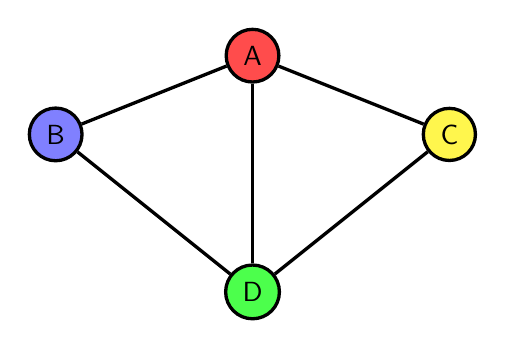
\begin{tikzpicture}
						\node[red-node] (A) at (2.5,5) {A};
						\node[blue-node] (B) at (0,4) {B};
						\node[yellow-node] (C) at (5,4) {C};
						\node[green-node] (D) at (2.5,2) {D};
						
						\path [-] (A) edge (B);
						\path [-] (A) edge (C);
						\path [-] (A) edge (D);
						\path [-] (B) edge (D);
						\path [-] (D) edge (C);
					\end{tikzpicture}
					\caption{4 colors}
				\end{subfigure}%
				\begin{subfigure}{.5\textwidth}
					\centering
		    		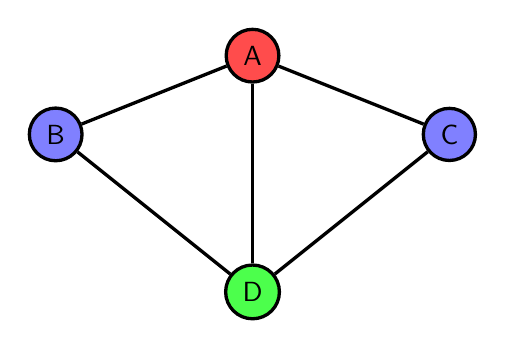
\begin{tikzpicture}
						\node[red-node] (A) at (2.5,5) {A};
						\node[blue-node] (B) at (0,4) {B};
						\node[blue-node] (C) at (5,4) {C};
						\node[green-node] (D) at (2.5,2) {D};
						
						\path [-] (A) edge (B);
						\path [-] (A) edge (C);
						\path [-] (A) edge (D);
						\path [-] (B) edge (D);
						\path [-] (D) edge (C);
					\end{tikzpicture}
					\caption{3 colors}
				\end{subfigure}
			
				\caption{Chromatic number}
				\label{fig:1}
			\end{figure}
			
	\pagebreak
			
	\chapter{Solution Overview}
	
    	\section{Computational Complexity}
    	
    		\begin{figure}[h]
    			\centering
    			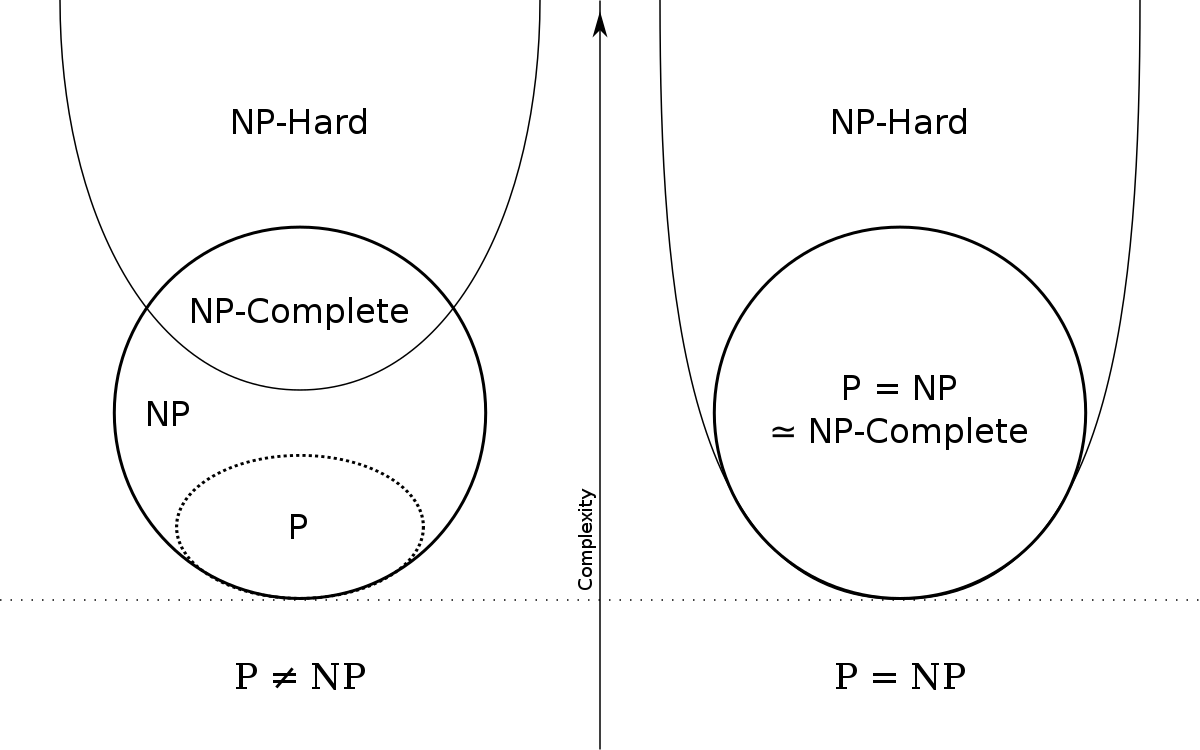
\includegraphics[scale=0.5,width=0.8\linewidth]{diagrams/diagram-3.png}
    			\label{fig:3}
    		\end{figure}
    	
	    	The graph coloring problem is a computationally difficult problem. The problem can be stated in two ways 
	    	\vspace{20pt}
    		
    		\begin{enumerate}
    			\item 
	    			\textbf{Decision Problem}: \textit{``Can the graph be colored using $k$ colors?''} \vspace{5pt} \\
	    			NP contains the set of problems for which the correctness of any solution can be verified in polynomial time. And NP-complete is the subset of the most difficult problems within NP. This decision problem is NP-Complete because if we are given a coloring it can be checked in polynomial time whether or not it uses less than $k$ colors.
	    			
	    \pagebreak
	    
    			\item 
	    			\textbf{Optimization Problem}: \textit{``What is the minimum number of colors needed to color a graph?''} \vspace{5pt} \\ 
	    			Even if we are given a coloring, we will not be able to verify in polynomial time whether it's the minimum. This is an NP-Hard problem. These problems are as hard as the hardest problems in NP. 
    		\end{enumerate}
	
    	\section{Algorithmic Paradigms}
    	\vspace{20pt}
    	
    		As it is a computationally hard problem there are two different approaches to solving it. Both has its own advantages, disadvantages and specific use cases. They are briefly described below:
    		\vspace{20pt}
    		
    		\begin{enumerate}
    			\item 
    			\textbf{Approximate algorithms}: These are solvable in polynomial time. But these algorithms can not guarantee an optimum value i.e. minimum value of chromatic number. Greedy algorithms fall under this paradigm. These algorithms can be used in practical scenarios where some error can be sacrificed to get faster results. \\
    			\item 
    			\textbf{Exact algorithms}:  These algorithms can guarantee optimal results. But they take exponential time which is not practical for bigger graphs. Examples of such algorithms include dynamic programming algorithms. These solutions might only be practical under certain constraints placed in the graph e.g. bipartite graphs, perfect graphs, planar graph with low branch-width, etc. In general, the time required is polynomial in the graph size, but exponential in the branch-width.  \\
    		\end{enumerate}
    	
    	\pagebreak
	
	\chapter{Greedy Algorithm}
	
    	\section{Basic Idea}	
    		The fundamental idea of a greedy algorithm is to make locally optimal choice at each step. This is called the \textit{greedy choice} and making such a choice at each step ultimately yields a globally optimum solution. \vspace{20pt} \\
    		\textbf{Greedy choice:} For our graph coloring problem, when we encounter a new node $V_i$ we should try to use existing colors (from our list of colors $C$) instead of introducing a new color. But the existing color should not already be present in the list of nodes $\varepsilon$ adjacent to $V_i$. \vspace{20pt}
    		
    		\begin{itemize}
    			\item A color exists in the list which is not present in any adjacent node $k$
    			\begin{equation}
    			\label{eqn:1}
    			V_i.color = k : (k \in C) \hspace{5pt} \& \hspace{5pt} (k \not\in \varepsilon)
    			\end{equation}
    			
    			
    			\item If all existing colors are present in adjacent we introduce a new color
    			\begin{equation}
    			\begin{aligned}
        			\label{eqn:2}
        			V_i.co & lor = k : (k \not\in C) \\
    			    C & = C \cup \{k\}
    			\end{aligned}
    			\end{equation}
    		\end{itemize}
    	
    		\pagebreak
	
    	\section{Algorithm}
				
		\begin{figure}[h]
            \centering
            \begin{subfigure}[t]{0.45\textwidth}
                \centering
                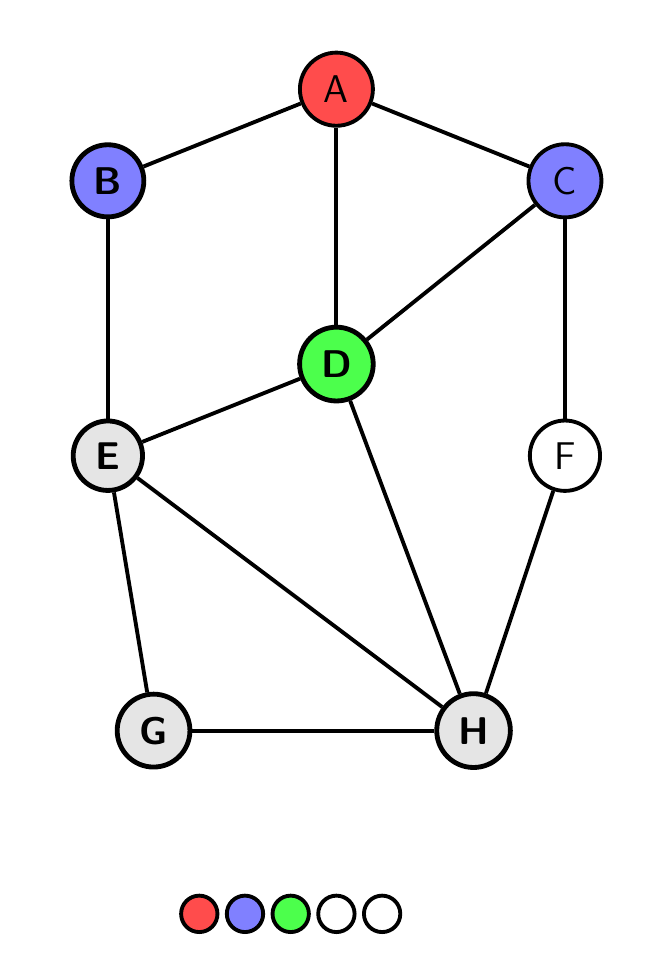
\includegraphics[width=0.9\linewidth]{diagrams/greedy-1.png}
                \subcaption{}
            \end{subfigure}
            \hfill
            \begin{subfigure}[t]{0.45\textwidth}
                \centering
                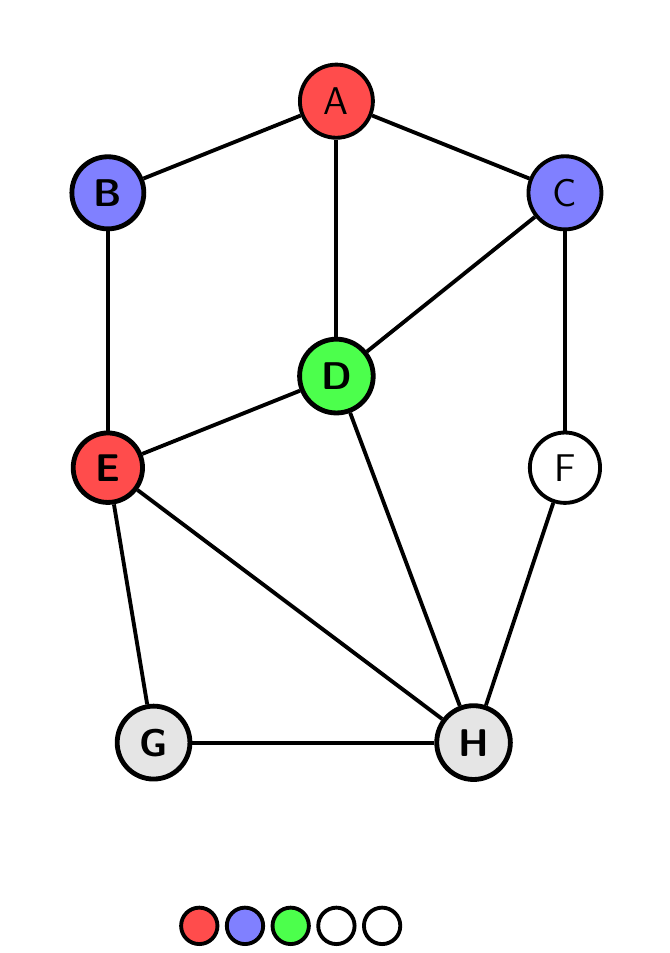
\includegraphics[width=0.9\linewidth]{diagrams/greedy-2.png}
                \subcaption{}
            \end{subfigure}
            \caption{\textbf{Simulation of greedy choice}}\
            \label{fig:1}
        \end{figure}\
        
        The algorithm starts off with the graph and list of all colors $C$. We color nodes A, B, C and D and arrive at node E. We take a look at the adjacent nodes B, D, G and H. We have a color (red) left in our list $C$ which was previously used but not present in any adjacent nodes. So we reuse that color instead of introducing a new one. This is the basis of our greedy choice and we continue until the whole graph is colored using 3 colors and that is our chromatic number.
        
        \pagebreak
    	
    	\begin{algorithm}[ht]
    	    \ttfamily
		    \caption{GREEDY(G)}
		    \SetKwInOut{Input}{Input}
		    \SetKwInOut{Output}{Output}
            \Input{A Graph G}
            \Output{Chromatic Number of G}
            
            list of used colors, $C = \emptyset$ \\
            \For{$i=1$ to $V(G)$}{
                $\epsilon = \emptyset $\\
                \For{$j \in Adj(V[i])$}{
                    $\epsilon$ $\cup$ color$[j]$
                }
                \If{$C == \epsilon$}{
                    $k = $new color \\
                    $C = C \cup k$
                }
                \Else{
                    $k = (C \setminus \epsilon)[0]$
                }
                Color $V[i]$ with k
            }
            \Return{length of $C$}
		\end{algorithm}
	
    	\section{Complexity \& Limitations}
    	
    		\vspace{20pt}
   			The time complexity is $O(V^2 + E)$ in the worst case. \\
   			
   			The algorithm \textbf{doesn't always use the minimum number of colors}. Actually the number of colors used depends on the order in which the vertices are processed. Different ways of picking vertices have been suggested but the most common in \textit{Welsh-Powell} algorithm which considers vertices in decending order of degrees \\ 
   			
   			A vertex might be connected to at most $d$ vertices which means at most $d$ colors might've been used by its adjacents and we introduce a new color. This \textbf{guarantees an upper bound of $d+1$} on the chromatic number where $d$ is maximum degree of the graph.
    	
    		\pagebreak
	
	\chapter{Dynamic Programming}
	
	\section{Basic Idea}	
		Dynamic Programming (DP) is an algorithmic technique for solving an optimization problem by breaking it down into simpler sub-problems and utilizing the fact that the optimal solution to the overall problem depends upon the optimal solution to its sub-problems. A problem must have 2 attributes to be eligible for this technique: 
		\begin{itemize}
		    \item Optimal sub-structure
		    \item Overlapping sub-problem
		\end{itemize}
		
		\vspace{10pt} 
		
		\subsubsection*{Graph DP properties}
		In accordance to dynamic programming problem attributes, the graph coloring  problem also exhibits the 2 aforementioned properties. If a graph $G$ with $4$ vertices is considered, then the chromatic number of $G$ can be derived utilizing the chromatic numbers of $S$ which are subgraphs of $G$ containing $3$ or less vertices. Thus by extracting the solutions of sub-graphs, we can retrieve the solution of the whole graph. 
		\\
		
		\subsubsection*{Maximal Independent Sets}
		An Independent set is a set of vertices such that any two vertices in the set do not have a direct edge between them. Consequently, a maximal independent set is an independent set having highest number of vertices. Thus a maximal independent set can be colored using a single color as they do not share any direct connecting edge. So a maximal independent set is 1-colorable.
		\\
		
		\pagebreak
		
		\subsubsection*{Lawler's Solution}
		Lawler\cite{LAWLER197666} was the first to propose a dynamic programming algorithm for the graph coloring problem. He observed that \emph{Every graph has an optimal coloring in which (at least) one of the colors is a maximal independent set}. If $G$ is a graph with $V$ vertices and $S \subseteq V(G)$, then $\chi(G[S])$ or the chromatic number of $G$ is the minimum among $1+\chi(G[S])$ over all maximal independent sets $I$ in $G[S]$. The relation can be defined as:
		
		 \[ 
		  \chi(G[S]) = \begin{cases} 
              0 & S = \emptyset\\
              1 + min(\chi(G[S\setminus I]))  & S \neq \emptyset
           \end{cases}
        \]
        
        Thus by always taking the minimum at each subgraph, the chromatic number of the whole graph can be derived. 
	
		\section{Algorithm}
		This algorithm always returns the exact chromatic number of a graph utilizing the dynamic programming properties.
		
		
		\begin{algorithm}[ht]
		    \ttfamily
		    \caption{LAWLER(G)}
		    \SetKwInOut{Input}{Input}
		    \SetKwInOut{Output}{Output}
            \Input{A Graph G}
            \Output{Chromatic Number of G}
            $n = |V(G)|$ \\
            $\chi = $ array indexed from $0$ to $2^n-1$ \\
            $\chi[0] = 0$ \\
            \For{$s=1$ to $2^n-1$}{
                $\chi[s] = \infty $\\
                \For{$i \in I(G(s))$}{
                    \If{$\chi[s \setminus i] + 1 < \chi[s]$}{
                        $\chi[s] = \chi[s \setminus i] + 1$
                    }
                }
            }
            \Return{$X[2^n-1]$}
    
		\end{algorithm}
		
		\pagebreak
		
		\begin{figure}[t]
        \centering
        \begin{subfigure}[t]{0.45\textwidth}
            \centering
            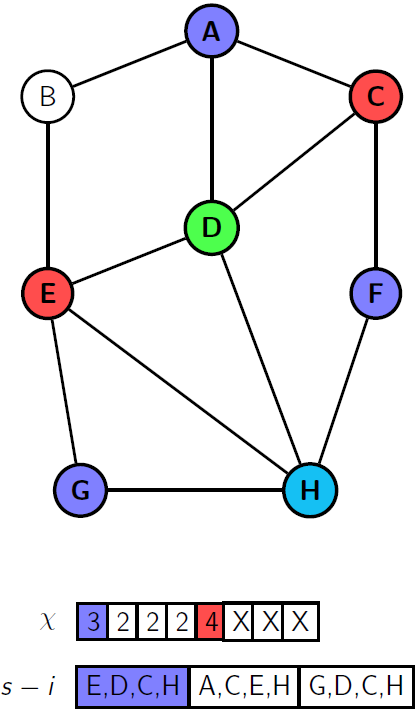
\includegraphics[width=0.9\linewidth]{diagrams/dp1.PNG}
            \subcaption{}
        \end{subfigure}
        \hfill
        \begin{subfigure}[t]{0.45\textwidth}
            \centering
            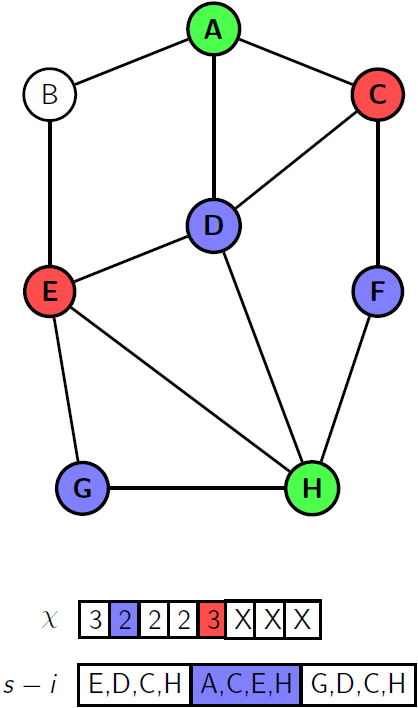
\includegraphics[width=0.9\linewidth]{diagrams/dp2.PNG}
            \subcaption{}
        \end{subfigure}
        \caption{\textbf{Simulation of Lawler's algorithm}}\
        \label{fig:1}
    \end{figure}\
    
    For example, the subgraph $ACDEFGH$ is considered. $AFG$ constitutes a maximal independent set. The remaining vertices $EDCH$ is 3 colorable. So $ACDEFGH$ must be $3+1$ or $4$ colorable. The same subgraph has another maximal independent set $DFG$. But this time, the remaining vertices $ACEH$ are 2 colorable. So we get an even lower chromatic number $2+1$ or $3$ which is $\chi(G[S])$
    
    \pagebreak
	
	\section{Complexity \& Limitations}
	    \vspace{20pt}
	    This algorithm has a running time of $O(2.4423^n)$ \cite{article}. Eppstein \cite{DBLP:journals/corr/cs-DS-0011009} modified  this algorithm to decrease the running time to $O(2.4150^n)$. Byskov \cite{Byskov} further developed this algorthim to lower the running time to $O(2.4023^n)$. \\
	    
	    These methods always give the \textbf{exact answer} but as their time and space complexity are of an exponential nature, they \textbf{cannot be realistically applied for large graphs}. On the other hand, these can be easily applied to smaller graphs.\\
	    
	    So there is an accuracy vs latency trade-off to consider before finalizing which technique to utilize in real life problems.
	
	\pagebreak
	
	\chapter{Applications}
	
    	\section{Map Coloring}
    	    In order to differentiate between neighboring countries or states or regions, they need to be colored differently. This problem is easily transferrable to graph coloring.
    	
    		\begin{figure}[h]
    		    \centering
    			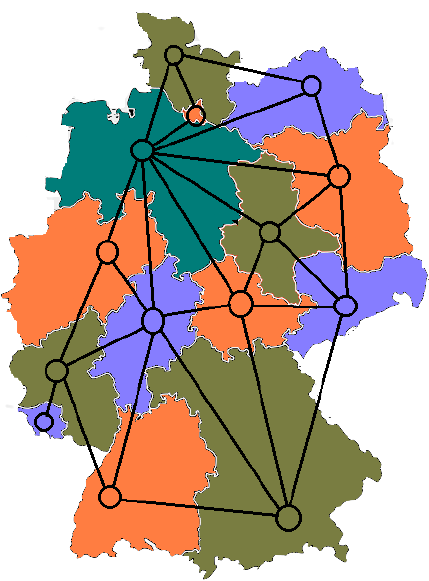
\includegraphics[scale=0.5]{diagrams/maps.png}
    			  \caption{Map Coloring}
    			\label{fig:maps}
    		\end{figure}
    		
    		By considering each country or state as a vertex of a graph, a map can be colored in such a way that no two neighboring regions will have the same colors.
    		
    		\pagebreak
    		
    		
    	\section{Register Allocation}
    	   \vspace{20pt}
    	    The number of registers in a computer architecture are generally kept on the low side to decrease cost. So an efficient method to utilize all registers to store currently active variables is needed. 
    		\begin{figure}[ht]
    			
    			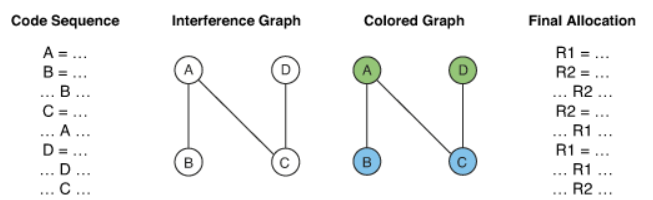
\includegraphics[scale=1.0]{diagrams/register_cropped.png}
    			  \caption{Efficient register allocation}
    			\label{fig:regs}
    		\end{figure}
    		\vspace{1cm}
    		
    		We cannot store 2 variables in the same register if their values depend on each other. This dependency can be modelled by making the variables vertices of a graph and adding an edge between them. Now it is easily solvable using the graph coloring solution.
	
    	\section{Scheduling Tasks}
    	    Similarly, by considering events or tasks as vertices of a graph and adding an edge between two vertices if they have overlapping time periods or other conflicts, the scheduling task problem can easily be converted into a graph coloring problem.
        
	\pagebreak
	
	\chapter{Conclusion}
	
	The decision to select an algorithm to solve the graph coloring problem in real life is done via considering all the trade-offs of each methods and the criteria of the problem solution. If a solution demands to be exact in all cases where there is no time constraint, then a variant of exact solutions can be used. But if the accuracy constraint is relaxed but the time limit is tightened, then an approximate solution can be utilized. Therefore we must consider both the capabilities and limitations for our approach and choose the right implementation for our specific cases.
	
	\pagebreak
	
	\nocite{*} 
	\printbibliography
	
	% %EFFECTS DEMO
	% \begin{frame}{Second Section: Frame 2}
	% This is a sample line of text.
	
	% \begin{itemize}
	%  \item<1-> Text visible from slide 1 
	%  \item<2-> Text visible from slide 2
	%  \item<3> Text visible on slide 3
	%  \item<4-5> Text visible on slides 4 and 5
	%  \item<5-> Text visible from slide 5
	%  \item<6-> Text visible from slide 6
	% \end{itemize}
	% \end{frame}
	
	% %EFFECTS DEMO USING PAUSE
	% \begin{frame}{Second Section: Frame 3}
	%  In this slide \pause
	
	%  the text will be partially visible \pause
	
	%  And finally everything will be there
	% \end{frame}
	
	% %TWO COLUMN SLIDE
	% \begin{frame}{Second Section: Frame 4}
	
	% \begin{columns}
	% \column{0.5\textwidth}
	% This is a text in the first column.
	% $$E=mc^2$$
	% This is a list.
	% \begin{itemize}
	% \item First item
	% \item Second item
	% \end{itemize}
	
	% \column{0.5\textwidth}
	% This text will be in the second column.
	% This is a nice looking
	% layout in some cases.
	% \end{columns}
	% \end{frame}
	
	% %BLOCK AND ALERT COMMANDS
	% \begin{frame}{Second Section: Frame 5}
	
	% In this slide, some important text will be
	% \alert{highlighted} because it's important.
	
	% \begin{block}{Remark}
	% Sample text
	% \end{block}
	
	% \begin{alertblock}{Important theorem}
	% Sample text in red box
	% \end{alertblock}
	
	% \begin{examples}
	% Sample text in green box. 
	% \end{examples}
	% \end{frame}
	
\end{document}